\documentclass[11pt]{article}
\usepackage{amsmath}
\usepackage[margin=0.68in]{geometry}
\usepackage{booktabs}
\usepackage{enumitem}
\usepackage{fancyhdr}
\usepackage{graphicx}
\usepackage[table]{xcolor}
\usepackage[hidelinks]{hyperref}
\usepackage{listings}
\usepackage{microtype}
\usepackage{tabularx}
\usepackage{titlesec}
\graphicspath{{docs/lessons/assets/}{../assets/}}

\definecolor{Ink}{gray}{0}
\definecolor{CodeGray}{gray}{0.96}
\hypersetup{
  hidelinks,
  pdftitle={ADK Lesson 035: Passage Qualification},
  pdfauthor={Kevin Shanahan},
  pdfsubject={Deterministic passage dwell, direction, timeout, suppression, and evidence faults},
  pdflang={en-US}
}
\pagestyle{fancy}
\fancyhf{}
\lhead{\textsc{ADK Lesson 035}}
\rhead{Passage Qualification}
\cfoot{\thepage}
\setlength{\headheight}{14pt}
\setlength{\parindent}{0pt}
\setlength{\parskip}{5pt}
\setlist{nosep,leftmargin=1.45em}
\titleformat{\section}{\Large\bfseries\color{Ink}}{\thesection}{0.5em}{}
\lstdefinestyle{adkcpp}{
  language=C++, backgroundcolor=\color{CodeGray},
  basicstyle=\ttfamily\small, keywordstyle=\color{Ink}\bfseries,
  commentstyle=\color{Ink}, columns=fullflexible, keepspaces=true,
  showstringspaces=false, frame=single, rulecolor=\color{Ink},
  breaklines=true, tabsize=4
}
\newcommand{\lessonbox}[1]{%
  \begin{center}\fcolorbox{Ink}{white}{\parbox{0.92\linewidth}{#1}}\end{center}}

\begin{document}
\begin{center}
  {\Huge\bfseries Passage Qualification}\\[4pt]
  {\Large Turn two healthy boundaries into one bounded record}\\[8pt]
  \textit{Dwell first, decide once, suppress duplicates}
\end{center}

\begin{tabularx}{\linewidth}{@{}>{\bfseries}l X >{\bfseries}l X@{}}
Lesson & 035 --- component & Time & 120--180 minutes\\
Prerequisites & Lessons 032 and 034 & Board & Mega 2560 evidence panel\\
Evidence & TP-A, TP-B, three LED witnesses & Status & host verified; bench open\\
Energy class & E0 software fixture; no sensor connection or actuation\\
\end{tabularx}

\lessonbox{\textbf{Scope gate.} \texttt{PassageQualifier} is pure software. It
owns no pin, clock, endpoint, storage, callback, sensor, motor, gate, or lock.
TP-A and TP-B in the canonical sketch are deterministic fixture frames, not
electrical inputs. Do not connect a magnetic-family specimen until Lesson
034's exact-revision qualification and schematic gates are complete.}

\section{Mission and evidence chain}

The lesson preserves:
\[
\text{two healthy observations}\rightarrow\text{qualified boundary order}
\rightarrow\text{one passage record}.
\]
By the end, you can explain why a passage needs continuous dwell at two
geometric boundaries; distinguish accepted, timed-out, ambiguous, suppressed,
and faulty evidence; and prove that optional position corroborates direction
without becoming passage authority.

\section{Build the visible story in stages}

\begin{center}
% ADK visual: pencil
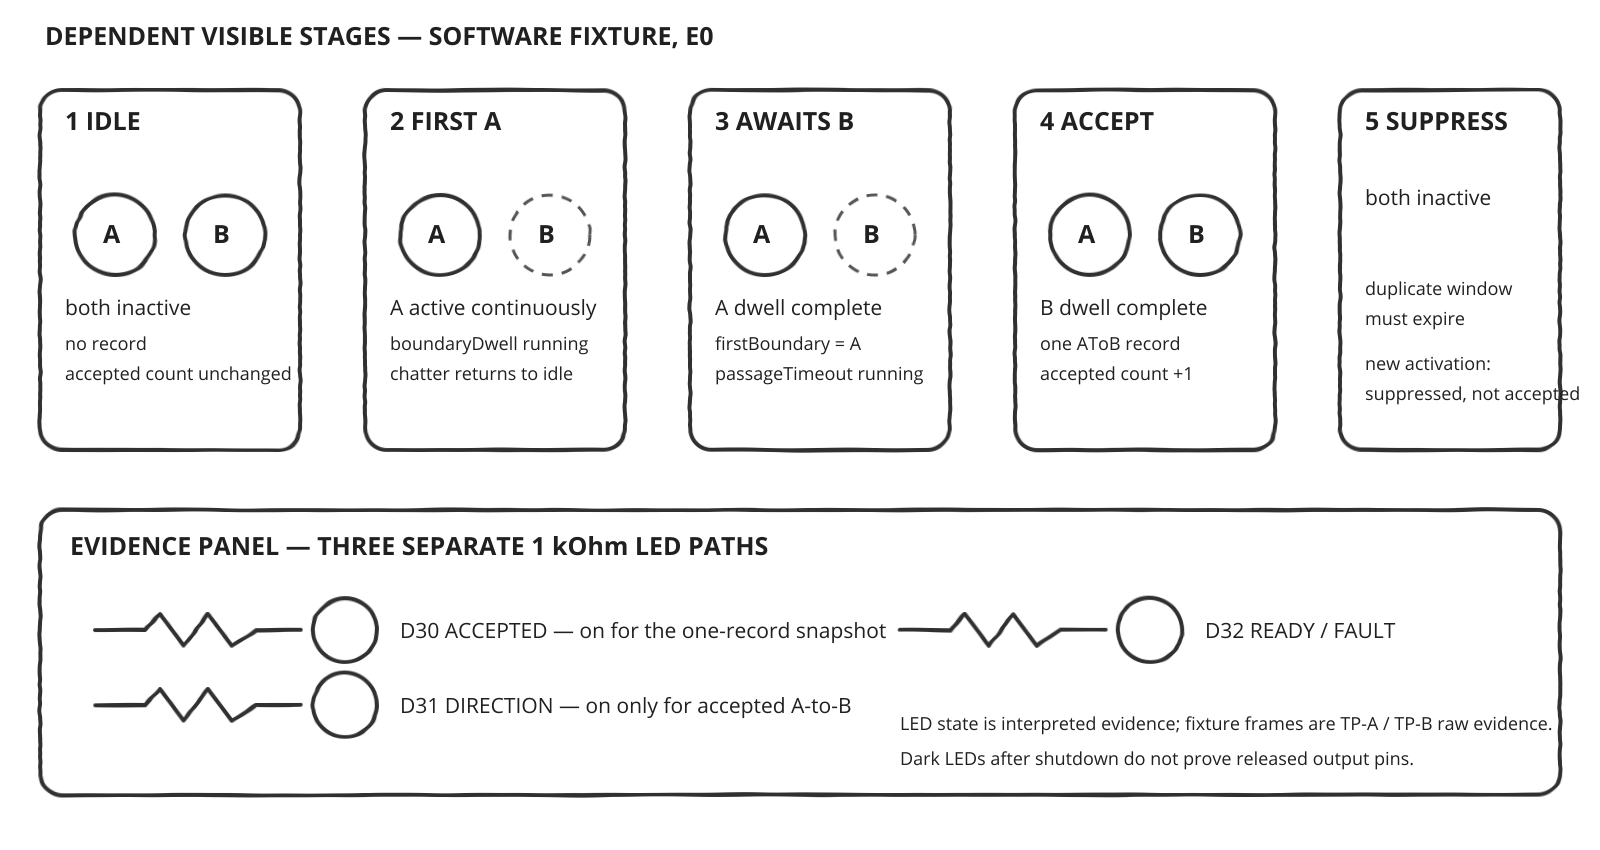
\includegraphics[width=0.98\linewidth]{035-passage-stages-pencil.png}

\small\textit{Alternative text: five pencil stages show Idle, boundary A
dwell, AwaitingSecond, one accepted A-to-B record, and duplicate suppression;
below, D30 shows accepted, D31 distinguishes accepted A-to-B, and D32 shows
ready versus fault through separate 1 k\(\Omega\) LED paths.}
\end{center}

Run the canonical software fixture with only the three resistor-limited LEDs.
First prove D32 ready. Then watch one A-to-B record light D30 and D31. The
later B-to-A record lights D30 without D31. Qualifier timestamps advance in
10 ms steps while each frame remains board-visible for 250 ms. This makes the
direction contrast human-readable without changing qualification time or
using Serial or an unidentified sensor.

\begin{tabularx}{\linewidth}{@{}l l X@{}}
\toprule
Evidence & Provisional panel role & Interpretation\\
\midrule
TP-A, TP-B & internal fixture trace labels & copied boundary activity and time; not board pins\\
D30 & LED through 1 k\(\Omega\) & latest snapshot contains Accepted record\\
D31 & LED through 1 k\(\Omega\) & that accepted record is A-to-B\\
D32 & LED through 1 k\(\Omega\) & qualifier is not in Fault\\
\bottomrule
\end{tabularx}

These roles are not a sensor schematic. Each direct LED is bounded to at most
5 mA at 5 V, but darkness does not prove output-pin release. The sketch stops
and releases the evidence panel independently after 120 seconds.

\section{Public contract}

\texttt{PassageQualifierConfig} contains nonzero \texttt{boundaryDwell},
\texttt{passageTimeout}, and \texttt{duplicateWindow}; timeout is at least
dwell and every duration is below the unsigned half-range.
\texttt{PassageInput} carries one timestamp, two \texttt{MagneticObservation}
values, and optional copied position evidence.

\begin{tabularx}{\linewidth}{@{}l X@{}}
\toprule
Snapshot or record field & Meaning\\
\midrule
\texttt{phase}, \texttt{firstBoundary}, \texttt{elapsed} & current qualification state\\
\texttt{hasRecord}, \texttt{record.sequence} & one terminal record in this snapshot\\
\texttt{direction}, \texttt{disposition} & AToB/BToA and accepted/rejected reason\\
\texttt{onset}, \texttt{end} & retained qualification timestamps\\
\texttt{position} & copied onset/end/delta plus reliability and saturation\\
\texttt{acceptedCount}, \texttt{suppressedCount} & saturating evidence totals\\
\texttt{status} & lifecycle, time, or qualification result\\
\bottomrule
\end{tabularx}

\texttt{initialize()} validates policy; \texttt{update(input)} advances once;
\texttt{snapshot()} observes without consuming; and \texttt{reset()} returns
to the just-initialized state and clears history and counts. A record remains
for exactly the terminal snapshot and disappears on the next later update.

\section{Timing, direction, and suppression}

\begin{center}
% ADK visual: pencil
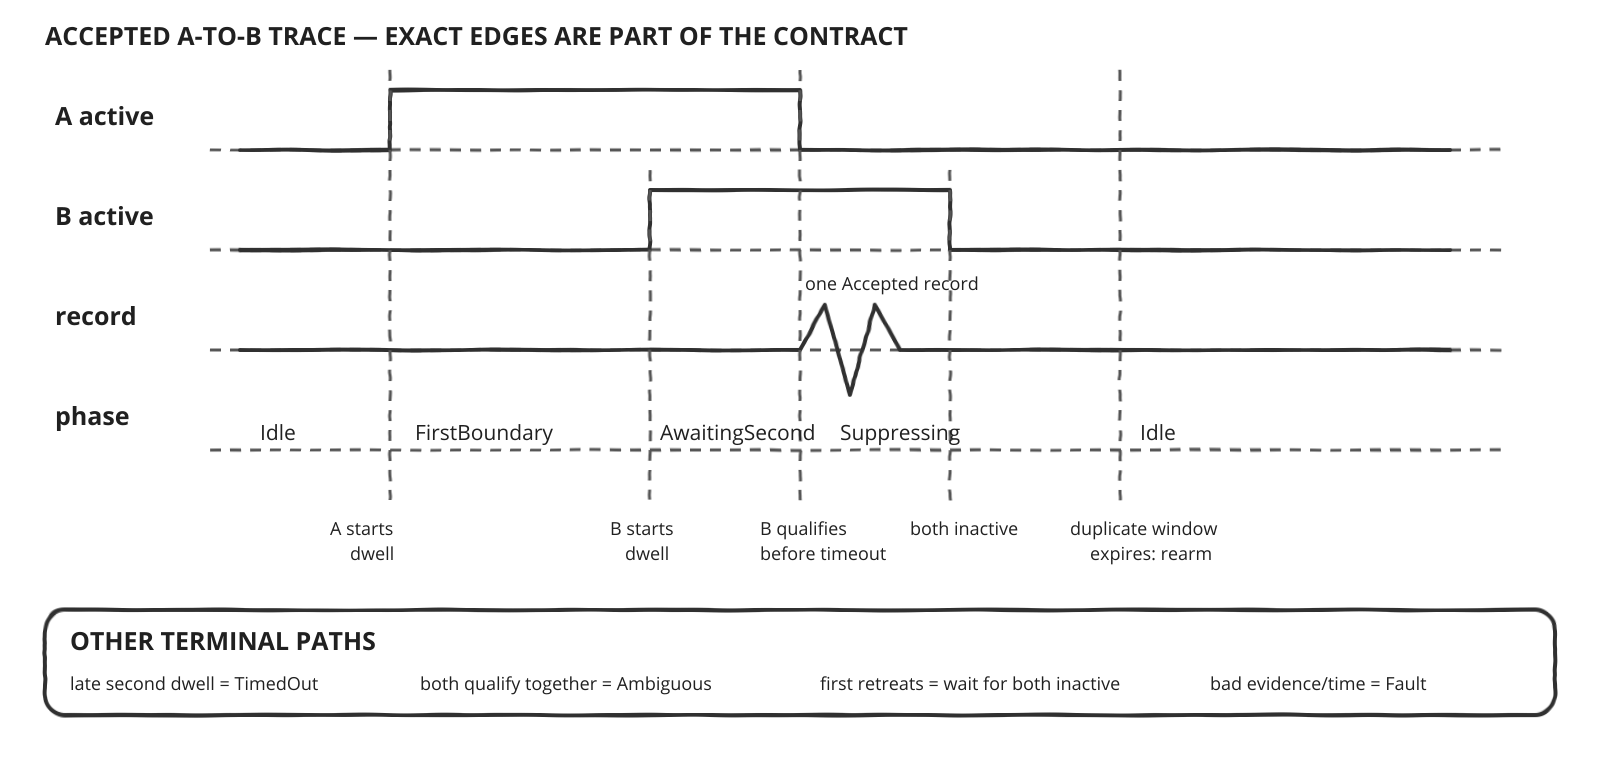
\includegraphics[width=0.98\linewidth]{035-passage-timing-pencil.png}

\small\textit{Alternative text: pencil timing tracks show A qualifying first,
B qualifying before the timeout edge, one accepted A-to-B record, and rearm
only after both boundaries are inactive and the duplicate window expires;
side cases name timeout, ambiguity, retreat, and fault.}
\end{center}

The timeout begins when the first boundary finishes dwell. The opposite
boundary may finish dwell at the exact timeout edge; a later completion times
out. Acceptance enters \texttt{Suppressing}. Rearm requires both inactive and
duplicate-window expiry. An activation inside that window emits one
\texttt{DuplicateSuppressed} record and increments only the suppressed count;
holding it active cannot count it again.

If the first boundary retreats before the second qualifies, the event cannot
reverse into acceptance. The qualifier waits until both are inactive, then
returns to Idle without a record. Simultaneous qualification is Ambiguous.

\section{Fault precedence and recovery}

Each input timestamp must equal both observation timestamps. Only observations
with Ok status and Valid quality participate. Precedence is invalid time,
source fault, ambiguity, timeout, then completion. An active candidate emits
one \texttt{EvidenceFault} record before entering Fault; an idle source fault
enters Fault without inventing a record. Recovery requires a later healthy
both-inactive frame and emits nothing.

Natural 32-bit rollover is valid. An exact half-range or larger apparent jump
faults without partial mutation. Repeating an identical same-time frame is
idempotent; changing any same-time evidence faults.

Optional position is corroboration only. A nonzero, unsaturated delta is
reliable when its sign agrees with A-to-B positive and B-to-A negative.
Missing, zero, opposite, source-failed, or saturated position remains explicit
but does not reject an otherwise accepted passage.

\section{Narrative Mega example}

\begin{lstlisting}[style=adkcpp]
void loop ()
{
    observeFixture ();

    if (!decidePassage () || !actuateEvidence ())
    {
        stopSafely ();
    }
}
\end{lstlisting}

The full sketch acquires the three witnesses, configures the qualifier, starts
the bounded fixture, and keeps observe--decide--actuate order. It creates
\texttt{MagneticObservation} fixture values in software and never reads a
physical sensor.

\section{Predict, observe, interpret}

\begin{enumerate}
  \item Predict D32 after successful initialization. Observe it separately
        from D30/D31; interpret it only as qualifier/panel readiness.
  \item Predict the first A dwell, later B dwell, direction, and exact record
        snapshot. Inspect the TP-A/TP-B fixture-trace columns (they are not
        board pins), then observe the board-visible D30/D31 pair.
  \item Reverse the trace. Predict D30 on and D31 off for accepted B-to-A.
  \item Place an activation inside suppression. Predict one suppressed record,
        no D30 accepted indication, and no accepted-count change.
  \item Inject timestamp mismatch in the host fixture. Predict Fault, then a
        silent recovery only on a later healthy both-inactive frame.
  \item Invoke shutdown. Predict dark LEDs, then verify released output state
        separately; LED darkness alone is insufficient.
\end{enumerate}

\section{Diagnosis and stop conditions}

\begin{tabularx}{\linewidth}{@{}X X@{}}
\toprule
Observation & Interpret and next check\\
\midrule
D30 never pulses & inspect dwell, timeout, health, and terminal snapshot timing\\
D31 disagrees & compare firstBoundary and accepted direction\\
repeated accepted pulses & inspect both-inactive and duplicate-window frames\\
Fault persists & supply a later healthy both-inactive frame\\
position unreliable & inspect presence, source status, sign, zero, and saturation\\
LED dark after stop & measure release; do not infer high impedance from darkness\\
\bottomrule
\end{tabularx}

\lessonbox{\textbf{Stop rule.} This lesson authorizes only the software fixture
and resistor-limited LED panel. Remove USB for heat, odor, reset, unstable
rail, unexpected LED state, or current-limit trip. Reconfigure only while
unpowered. Do not connect unknown specimens, motion, a gate, lock, vehicle,
launcher, ignition path, or safety system.}

\section{Exercises and software evidence}

\begin{enumerate}
  \item Draw the B-to-A counterpart of the accepted trace.
  \item Explain why retreat cannot become reverse acceptance.
  \item Order ambiguity, timeout, and completion at one timestamp.
  \item Explain why an unreliable position delta does not reject a passage.
  \item Give a rollover trace that completes boundary dwell across zero.
\end{enumerate}

Host tests cover both directions, exact dwell/timeout/suppression edges,
chatter, retreat, ambiguity, faults, recovery, same-time inputs, deterministic
replay, rollover, position reliability/saturation, reset, and saturating
sequences and counters. Compilation, tests, this PDF, and LED behavior are not
physical sensor acceptance.
The searchable HTML lesson is the primary accessible route. This PDF remains
untagged and makes no PDF/UA claim.

\end{document}
